Important: Neighborhoods, FLip and swap?. Search methods RW, BI, and FI (sidewalks). Heuristics obj var only and 
conflicting var only. Meta heuristic, Tabu search (tabu tenure, aspiration, Search procedure FI or BI, Neighborhood 
limitations for large neighborhoods?). Combining search procedure. \boste{Make overview of classes and methods} \\ \\ 
The \class{Local Search Engine} class uses the model created for local search described in section \ref{sec_ls} and 
uses local search to improve the initial solution. The optimization role of \class{Local Search Engine} is to create 
and manage neighborhoods and search procedure object. Neighborhoods and search procedures are combined to create 
different local search and \class{Local Search Engine} uses them within the time limit to improve the solution. \\ 
\begin{figure}[!b]
\begin{center}
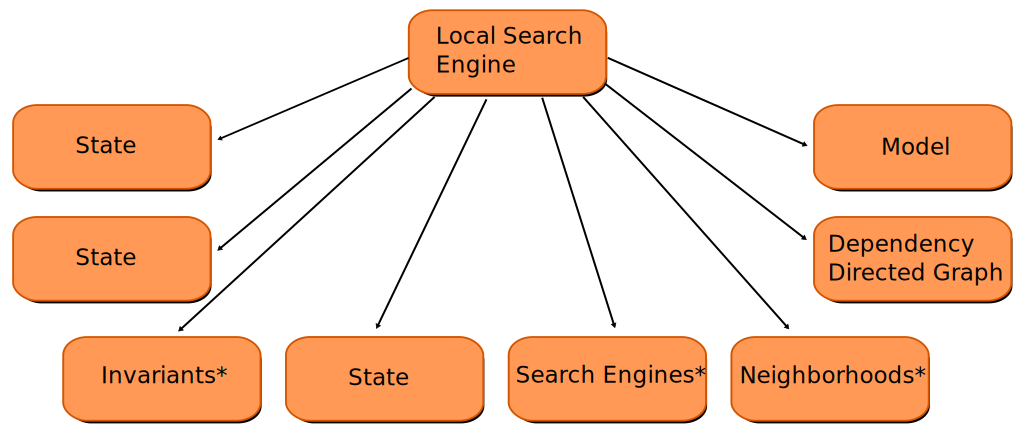
\includegraphics[width=0.9\linewidth]{LSE}\caption{Overview of the class pointers of Local Search Engine. The fields 
marked with a star (*) are several classes of that type.} 
\label{fig_lse}
\boste{Variable og constraint til venstre}
\end{center}
\end{figure}
The neighborhood classes are all subclasses of the super class \class{Neighborhood} such that they easily can be 
combined with the search procedures. The methods of neighborhoods is illustrated in figure \ref{fig_neighbborhood}. \\
\boste{Overview of methods of neighborhood} \\ 
Three neighborhoods are implemented, \class{FlipNeighborhood}, \class{MinConflictFlipNE}, and 
\class{EvalFlipNE}. 

The two latter are both flip neighborhoods but only consider the variables in violated 
constraints and in the variables in the evaluation function respectively. 
Neighborhoods defines the move type and an overall restriction of the independent variables in consideration, if any. 
The move type flip consist of a single binary variable $x$ and changes it value to $1-V(x)$. The 
\class{FlipNeighborhood} defines this neighborhood and the size of the neighborhood is $n'$, $n'$ is the number of 
independent variables.  
\boste{Skal være mere om hvad jeg har implementeret, ellers skal det skrives i section \ref{sub_lsalg}.}
Three different search procedures are implemented; first improvement, best improvement, and random walk. \\ 
First improvement look at neighbor solutions until a solution better than the current is found \boste{solution better 
than other?} and then make the move to reach that solution and returns true. When the search reaches a local optima no 
improving move can be found and first improvement returns false. As an alternative if no 
improving solution is found a move to solution of same quality could be made, called a sidewalk. It might be an 
improving solution can be found after a sidewalk. If sidewalks are allowed there must be some restriction to the 
sidewalks to prevent cycling through the same solution over and over. For instance this could be forbidding a number of 
consecutive sidewalks. The local optima could be reach very fast hence first improvement need to be complimented with 
other search procedures to continue the search. \\ 
Best improvement explores the whole neighborhood of the current solution and commits the move that gives the best 
improvement. It might take more time to explorer the neighborhood than first improvement but often find a 
better move than first improvement. If no improving move is found it does not commit a move and returns false. Like 
first improvement sidewalks could be allowed. \\ 
The neighborhood of a solution depends on the choice of move and heuristics applied to the neighborhood. The 
neighborhood implemented is \boste{are} 
